\documentclass{beamer}
\usepackage{tikz}

\begin{document}

\begin{frame}{¿Qué es \texttt{Musixtex}?}
    \begin{columns}[T]
        \column{0.4\textwidth}
            \begin{itemize}
                \item Some text A.
                \item Some text B.
                \item Some text C.
            \end{itemize}
        \column{0.6\textwidth}
            \centering
            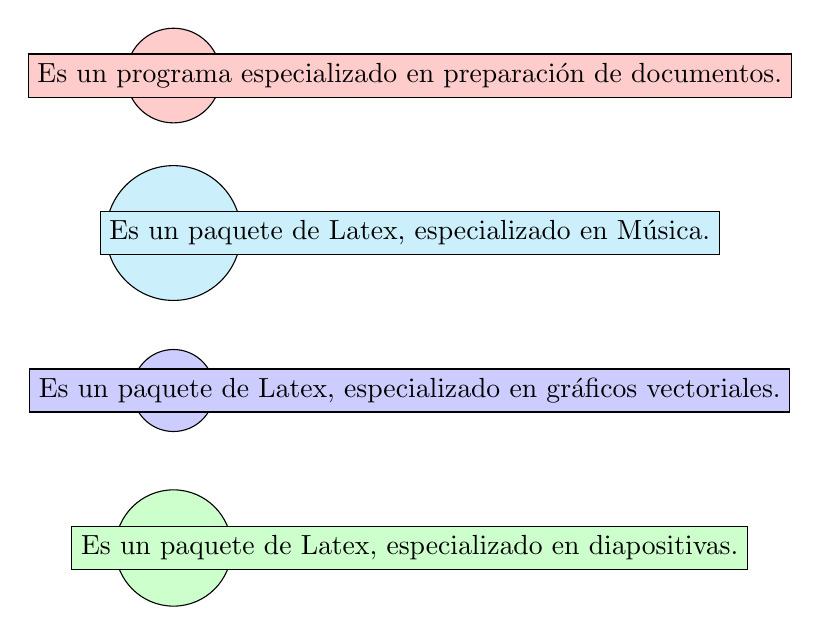
\begin{tikzpicture}[node distance=2cm]
                \node[draw,circle,fill=red!20] (latex) {Latex};
                \node[draw,circle,fill=cyan!20, below of=latex] (musixtex) {Musixtex};
                \node[draw,circle,fill=blue!20, below of=musixtex] (tikz) {Tikz};
                \node[draw,circle,fill=green!20, below of=tikz] (beamer) {Beamer};
                
                \node[draw,rectangle,fill=red!20, right of=latex, xshift=1cm] (latex_desc) {Es un programa especializado en preparación de documentos.};
                \node[draw,rectangle,fill=cyan!20, right of=musixtex, xshift=1cm] (musixtex_desc) {Es un paquete de Latex, especializado en Música.};
                \node[draw,rectangle,fill=blue!20, right of=tikz, xshift=1cm] (tikz_desc) {Es un paquete de Latex, especializado en gráficos vectoriales.};
                \node[draw,rectangle,fill=green!20, right of=beamer, xshift=1cm] (beamer_desc) {Es un paquete de Latex, especializado en diapositivas.};
            \end{tikzpicture}
    \end{columns}
\end{frame}

\end{document}